\section{Análisis de Borde y Asimetría}

En este apartado, la imagen sujeta a manipulación (Figura~\ref{fig01}) corresponde a un tumor canceroso maligno. Antes de abordar la técnica para resaltar los contornos mediante una imagen binaria, se llevará a cabo una manipulación inicial de la imagen con el propósito de obtener resultados más pobres. Este método implica la conversión de la imagen de su formato original en RGB a de grises. A través de una función de reducción de intensidad, se obtendrá una representación binaria de la imagen (Figura~\ref{fig02}).

\begin{figure}[h] 
	\begin{center} 
		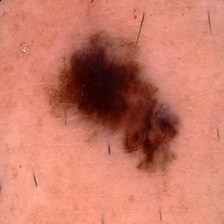
\includegraphics[width=4cm]{images/F01-A.png} 
	\end{center} 
	\vspace{-10pt}
	\caption{\footnotesize Melanoma maligno representado en el espacio RGB con una resolución de 224x244 píxeles almacenado en formato jpg.}  
	\label{fig01} 
\end{figure}

Podemos observar que en este primer método, los bordes se destacan de forma abrupta, obteniendo resultados poco suavizados y con una serie de disparos en el interior del área, los cuales nos gustaría evitar. Para mejorar esta propuesta, es posible segmentar el color de la imagen original mediante un algoritmo K-Means. Después de esta segmentación, se transforma la imagen a escala de grises. En esta etapa, reduciremos el rango dinámico para obtener una imagen binaria. Sin embargo, se observará que los resultados aún pueden mostrar cierta falta de suavidad en el contorno. Más adelante, se abordará una solución factible a este problema.

\begin{figure}[h] 
\begin{center} 
 \begin{tabular}{ccc}
        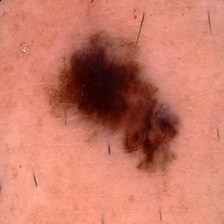
\includegraphics[width=2.4cm]{images/F01-A.png} &
        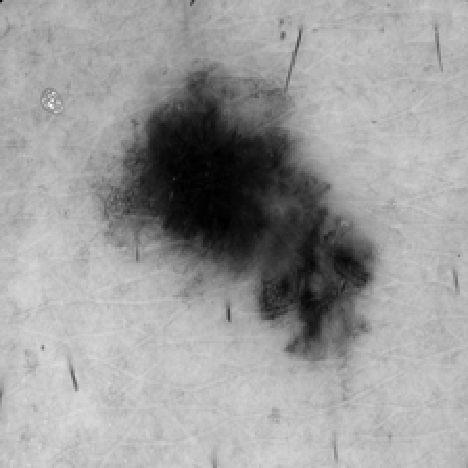
\includegraphics[width=2.4cm]{images/F01-B.png} & 
        
\includegraphics[width=2.4cm]{images/F01-C.png} \\
    (a) & (b) & (c)\\
  \end{tabular}
\end{center} 
\vspace{-10pt}
\caption{\footnotesize (a) Imagen original en el modelo RGB, (b) Imagen original en escala de grises, (c) Imagen en escala de grises con el rango dinámico reducido a dos valores (0 y 255).}  
\label{fig02} 
\end{figure}

\subsection{Implementación del Algoritmo K-Means}

La segmentación de color es una técnica utilizada en visión por computadora para identificar y distinguir diferentes objetos o regiones en una imagen basándose en sus colores \autocite{Anju:2019, Anju:2019, Dhanachandra:2015}. Los algoritmos de agrupamiento pueden separar automáticamente colores similares, sin necesidad de especificar valores de umbral para cada color. Esto puede ser útil al trabajar con imágenes que tienen una amplia gama de colores o cuando los valores de umbral exactos no se conocen de antemano \autocite{Bolat-2022}. 

El desarrollo completo de los algoritmos y métodos se llevará a cabo en MATLAB, por lo que se incorporarán fragmentos de código en este lenguaje. Inicialmente, definimos una función que requiere tres parámetros: la imagen original, el número deseado de grupos (indica la cantidad de tonalidades que tendrá la imagen resultante) y un número máximo de iteraciones para la segmentación. Dentro de la función se realizan las siguientes operaciones:

\begin{itemize}
    \item Se reorganiza la matriz originalImage en una nueva matriz con el número de filas igual al número total de elementos en originalImage y el número de columnas igual a 3 (una columna para cada canal de la imagen).
    \item De forma aleatoria, se seleccionan n índices de la matriz anterior, donde n corresponde al total de clústers. 
    \item En una nueva matriz ''centers'' de tres columnas se almacenan los valores de las $n$ posiciones aleatorias con los valores de los tres canales de color.
    \item Dentro de un ciclo for, en la variable ''D'' se calcula la distancia euclidiana entre los centros y cada píxel de la imagen, esto con ayuda de la función ''pdist2'' de MATLAB.
    \item Se actualizan los centros de los de los clústers. Para esto se crea un vector lógico donde todos los valores verdaderos son aquellos que pertenecen al cluster en ese punto de la iteración. Con esto, se pueden seleccionar todos los píxeles  de la imagen original que pertenecen a j. Por último se calcula la media de los píxeles seleccionados, esto actualiza el centro del cluster al promedio de las posiciones de los píxeles asignados a ese cluster.

    \begin{lstlisting}[style=Matlab-editor, caption=Fragmento del algoritmo K Means, basicstyle=\fontsize{8}{12}\selectfont]
    for iter=1:maxIter
        D = pdist2(centers,im2);
        [~,min_indices] = min(D);
        for j=1:clusterNo
            centers(j,:) = mean(im2(min_indices == j,:));
        end
    end
    \end{lstlisting}

    \item Se hace una asignación de colores a cada píxel según el cluster al que pertenece. Primero se  reorganiza la asignación de colores en la forma de la imagen original, se normalizan los valores de color a un rango de 0 a 1 y se acomodan en los tres canales de color.
\end{itemize}

De forma empírica se elige trabajar con 15 clústers y 100 iteraciones para el algoritmo. Las imágenes resultado donde este valor es ingresado de forma manual tendrán los valores mencionados. La imagen original en el modelo RGB (Figura~\ref{fig01}) segmentada con 15 clústers (Figura~\ref{fig03}) presenta ligeras variaciones en las tonalidades.

\begin{figure}[h] 
	\begin{center} 
		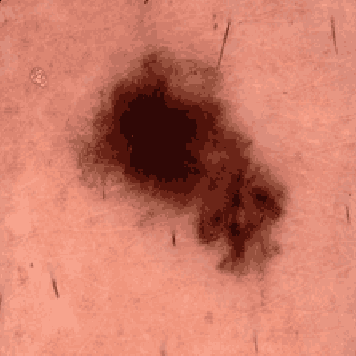
\includegraphics[width=4cm]{images/F03-A.png} 
	\end{center} 
	\vspace{-10pt}
	\caption{\footnotesize Imagen segmentada mediante el algoritmo K-Means con 15 clústers y 100 iteraciones.}  
	\label{fig03} 
\end{figure}

Si esta imagen la transformamos en una imagen en blanco y negro para después reducir su rango dinámico a dos, obtendríamos una imagen binaria con prevalecía de ruido en los alrededores y cambios abruptos en los bordes de la región principal (Figura~\ref{fig04}). Como solución a este problema se puede aplicar un filtro paso bajas butterworth a la imagen con el objetivo de suavizar y reducir elementos no deseados como lo son el ruido.  

\begin{figure}[h] 
\begin{center} 
 \begin{tabular}{cccc}
        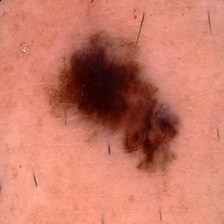
\includegraphics[width=1.7cm]{images/F01-A.png} &
        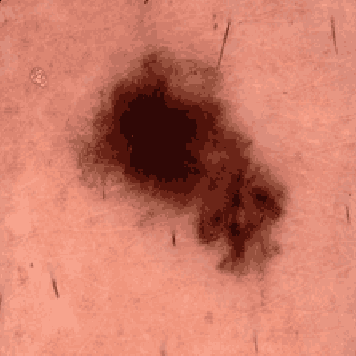
\includegraphics[width=1.7cm]{images/F03-A.png} & 
        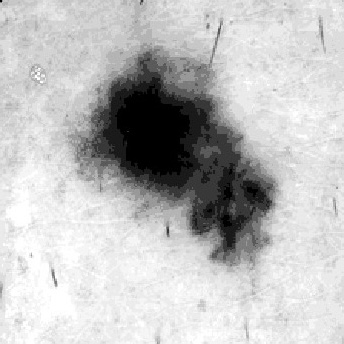
\includegraphics[width=1.7cm]{images/F04-A.png} & 
        
\includegraphics[width=1.7cm]{images/F04-B.png} \\
    (a) & (b) & (c) & (d)\\
  \end{tabular}
\end{center} 
\vspace{-10pt}
\caption{\footnotesize (a) Imagen original en el modelo RGB, (b) Imagen original segmentada en 15 clústers y 100 iteraciones, (c) Imagen segmentada en blanco y negro, (d) Imagen en blanco y negro con el rango dinámico reducido a dos valores.}  
\label{fig04} 
\end{figure}

\subsection{Implementación de un Filtro Paso Bajas Butterworth}

El filtro de paso bajas Butterworth se utiliza para suavizar la imagen en el dominio de la frecuencia. Elimina el ruido de alta frecuencia de una imagen digital y conserva los componentes de baja frecuencia \autocite{Makandar:2015, Gonzalez:2008}. Además sirve para suavizar la imagen mediante dos parámetros: frecuencia de corte y orden. En la evaluación de bordes, la implementación de este tipo de filtro será para suavizar el área alrededor del tumor para después obtener una imagen binaria a partir de este resultado, esperando obtener una silueta de color negro con el melanoma. 

\begin{figure}[h] 
\begin{tabular}{cc}
    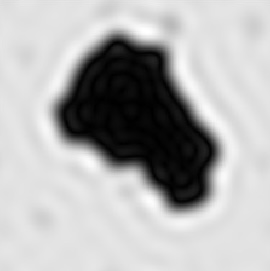
\includegraphics[width=1.7cm]{images/F05-A.png} &
    
\includegraphics[width=1.7cm]{images/F05-B.jpeg} \\
    FC: 10 & Orden: 10 \\
    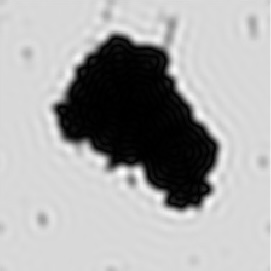
\includegraphics[width=1.7cm]{images/F05-C.png} & 
    
\includegraphics[width=1.7cm]{images/F05-D.jpeg} \\
    FC: 20 & Orden: 10 \\
    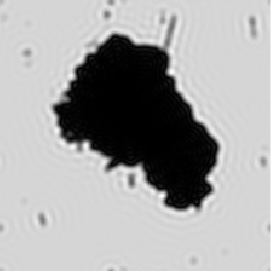
\includegraphics[width=1.7cm]{images/F05-E.png} &
    
\includegraphics[width=1.7cm]{images/F05-F.jpeg} \\
    FC: 30 & Orden: 10 \\
    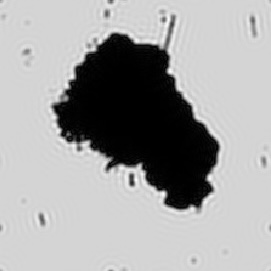
\includegraphics[width=1.7cm]{images/F05-G.jpeg} & 
    
\includegraphics[width=1.7cm]{images/F05-H.jpeg} \\
    FC: 40 & Orden: 10 \\
\end{tabular}
\vspace{10pt}
\caption{\footnotesize A, C, E y G representan segmentaciones en blanco y negro, sometidas a un filtrado de paso bajo de orden 10 con frecuencias de corte de 10, 20, 30 y 40, respectivamente. B, D, F y H son imágenes binarias derivadas de las segmentaciones correspondientes A, C, E y G.}  
\label{fig05} 
\end{figure}

Para las imagenes anexadas en este reporte se decide usar una frecuencia de corte de 20 con orden igual a 10. Estos valores pueden ser manipulados con diferentes parámetros con el objetivo de obtener resultados más suavizados. En (Figura~\ref{fig05}) se puede ver el comportamiento cuando el valor de la frecuencia de corte se va modificando, en la primera columna se encuentra la imagen con el filtro paso bajas y en la segunda la misma imagen con un rango dinámico reducido.

 \begin{figure}[h] 
	\begin{center} 
		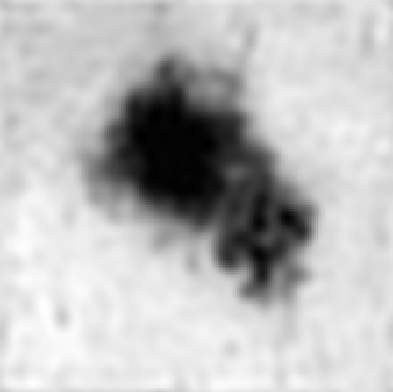
\includegraphics[width=4cm]{images/F06-A.png} 
	\end{center} 
	\vspace{-10pt}
	\caption{\footnotesize Melanoma maligno representado en escala de grises después de aplicar un filtro butterworth paso bajas de orden 10 con frecuencia de corte 20.}  
	\label{fig06} 
\end{figure}


En algunos casos el filtro es capaz de eliminar elementos no deseados que se encuentran situados en el exterior del área de interés. Esto aporta un gran valor sobre el resultado final pues es capaz de reducir filtraciones que dificulten diversos análisis como la evaluación de asimetría. Los resultados de este análisis abarcan desde la (Figura \ref{fig07}) hasta la (Figura \ref{fig11}).



\begin{figure*}
    \centering
    \begin{tabular}{cccccc}
        \adjustbox{valign=c}{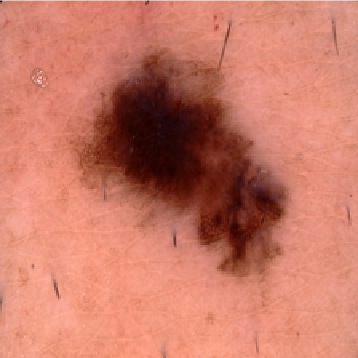
\includegraphics[width=1.7cm]{images/F07-A.png}} &
        \adjustbox{valign=c}{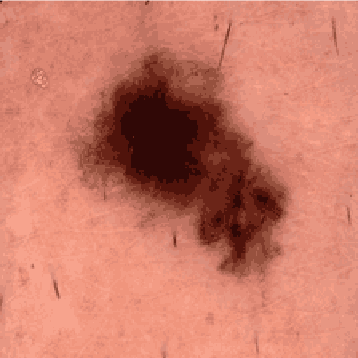
\includegraphics[width=1.7cm]{images/F07-B.png}} & 
        \adjustbox{valign=c}{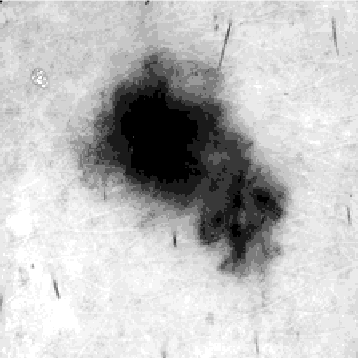
\includegraphics[width=1.7cm]{images/F07-C.png}} & 
        \adjustbox{valign=c}{
\includegraphics[width=1.7cm]{images/F07-D.png}} &
        \adjustbox{valign=c}{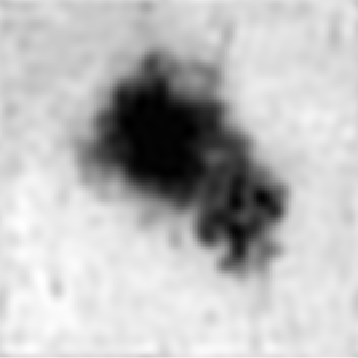
\includegraphics[width=1.7cm]{images/F07-E.png}} & 
        \adjustbox{valign=c}{
\includegraphics[width=1.3cm]{images/F07-F.png}} \\
        (a) & (b) & (c) & (d) & (e) & (f)\\
    \end{tabular}
    \caption{\footnotesize (a) imagen en el modelo RGB, (b) segmentación de color con K Medias, (c) imagen segmentada en blanco y negro, (d) imagen en blanco y negro con valores ecualizados, (e) imagen con valores ecualizados con trasnformación binaria, (f) imagen con filtro paso bajas.}  
    \label{fig07} 
\end{figure*}

\begin{figure*}
    \centering
    \begin{tabular}{cccccc}
        \adjustbox{valign=c}{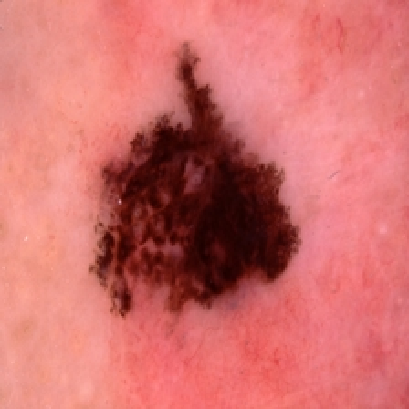
\includegraphics[width=1.7cm]{images/F08-A.png}} &
        \adjustbox{valign=c}{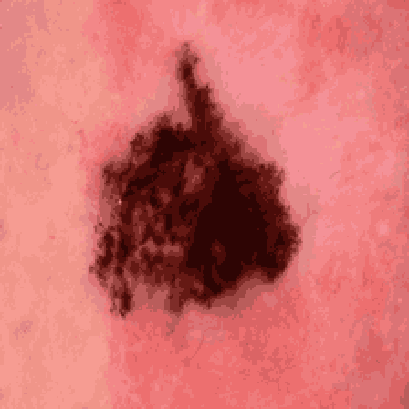
\includegraphics[width=1.7cm]{images/F08-B.png}} & 
        \adjustbox{valign=c}{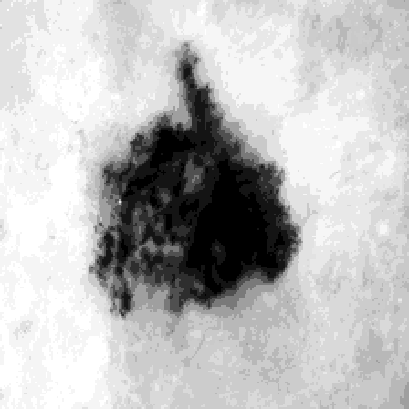
\includegraphics[width=1.7cm]{images/F08-C.png}} & 
        \adjustbox{valign=c}{
\includegraphics[width=1.5cm]{images/F08-D.png}} &
        \adjustbox{valign=c}{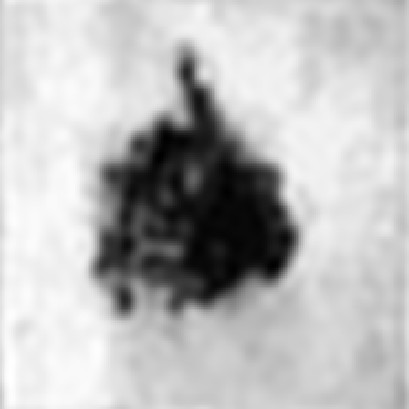
\includegraphics[width=1.7cm]{images/F08-E.png}} & 
        \adjustbox{valign=c}{
\includegraphics[width=1.3cm]{images/F08-F.png}} \\
        (a) & (b) & (c) & (d) & (e) & (f)\\
    \end{tabular}
    \caption{\footnotesize (a) imagen en el modelo HSI, (b) segmentación de color con K Medias, (c) imagen segmentada en blanco y negro, (d) imagen en blanco y negro con valores ecualizados, (e) imagen con valores ecualizados con trasnformación binaria, (f) imagen con filtro paso bajas.}  
    \label{fig08} 
\end{figure*}

\begin{figure*}
    \centering
    \begin{tabular}{cccccc}
        \adjustbox{valign=c}{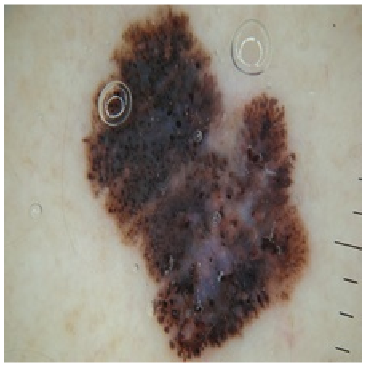
\includegraphics[width=1.7cm]{images/F09-A.png}} &
        \adjustbox{valign=c}{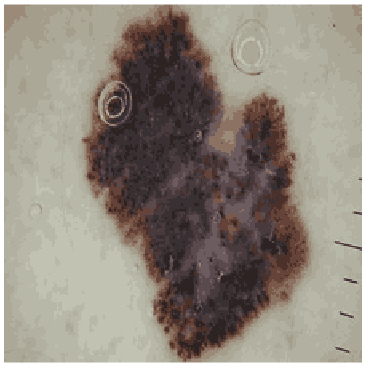
\includegraphics[width=1.7cm]{images/F09-B.png}} & 
        \adjustbox{valign=c}{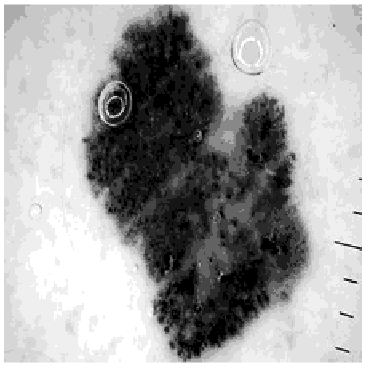
\includegraphics[width=1.7cm]{images/F09-C.png}} & 
        \adjustbox{valign=c}{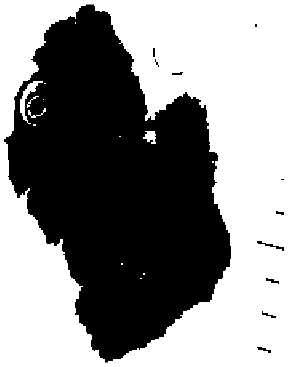
\includegraphics[width=1.2cm]{images/F09-D.png}} &
        \adjustbox{valign=c}{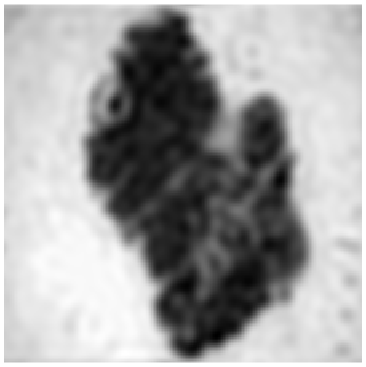
\includegraphics[width=1.7cm]{images/F09-E.png}} & 
        \adjustbox{valign=c}{
\includegraphics[width=0.9cm]{images/F09-F.png}} \\
        (a) & (b) & (c) & (d) & (e) & (f)\\
    \end{tabular}
    \caption{\footnotesize (a) imagen en el modelo HSI, (b) segmentación de color con K Medias, (c) imagen segmentada en blanco y negro, (d) imagen en blanco y negro con valores ecualizados, (e) imagen con valores ecualizados con trasnformación binaria, (f) imagen con filtro paso bajas.}  
    \label{fig09} 
\end{figure*}

\begin{figure*}
    \centering
    \begin{tabular}{cccccc}
        \adjustbox{valign=c}{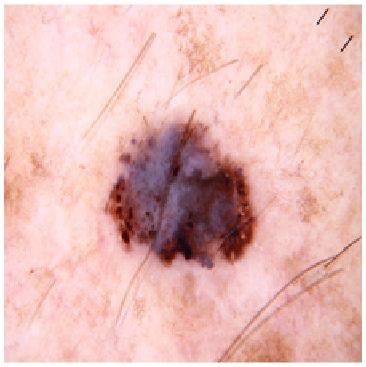
\includegraphics[width=1.7cm]{images/F10-A.png}} &
        \adjustbox{valign=c}{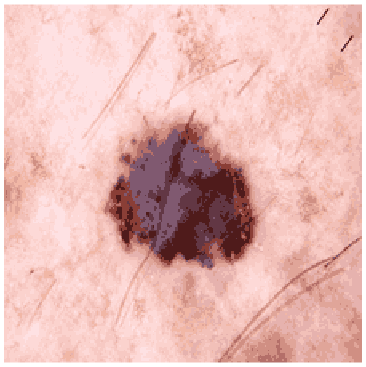
\includegraphics[width=1.7cm]{images/F10-B.png}} & 
        \adjustbox{valign=c}{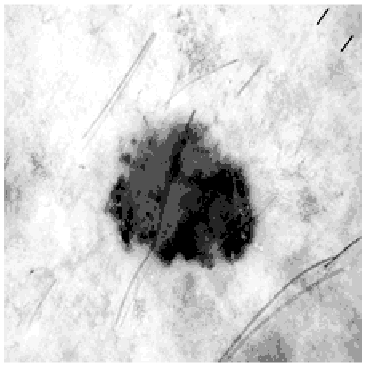
\includegraphics[width=1.7cm]{images/F10-C.png}} & 
        \adjustbox{valign=c}{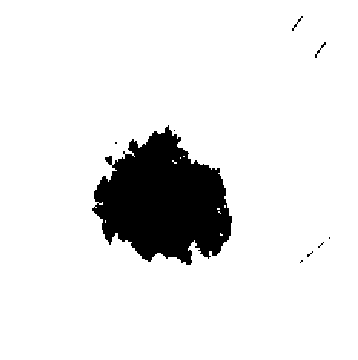
\includegraphics[width=1.7cm]{images/F10-D.png}} &
        \adjustbox{valign=c}{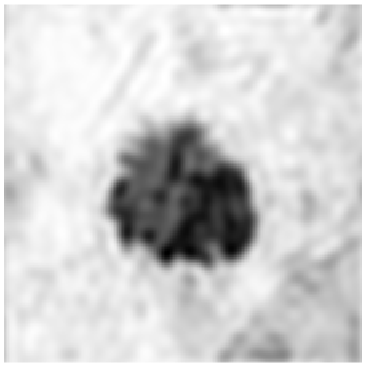
\includegraphics[width=1.7cm]{images/F10-E.png}} & 
        \adjustbox{valign=c}{
\includegraphics[width=0.8cm]{images/F10-F.png}} \\
        (a) & (b) & (c) & (d) & (e) & (f)\\
    \end{tabular}
    \caption{\footnotesize (a) imagen en el modelo HSI, (b) segmentación de color con K Medias, (c) imagen segmentada en blanco y negro, (d) imagen en blanco y negro con valores ecualizados, (e) imagen con valores ecualizados con trasnformación binaria, (f) imagen con filtro paso bajas.}  
    \label{fig10} 
\end{figure*}

\begin{figure*}
    \centering
    \begin{tabular}{cccccc}
        \adjustbox{valign=c}{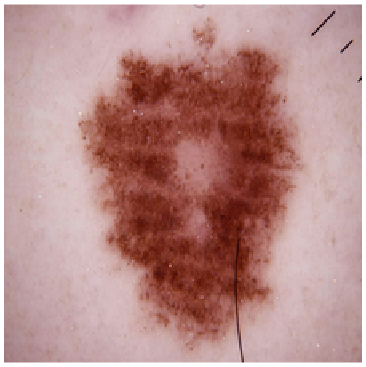
\includegraphics[width=1.7cm]{images/F11-A.png}} &
        \adjustbox{valign=c}{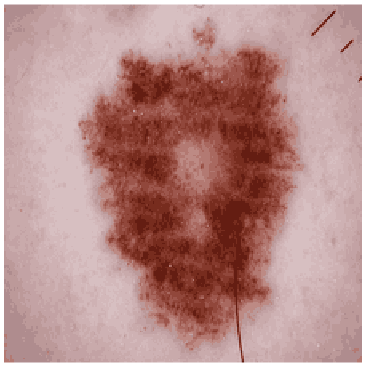
\includegraphics[width=1.7cm]{images/F11-B.png}} & 
        \adjustbox{valign=c}{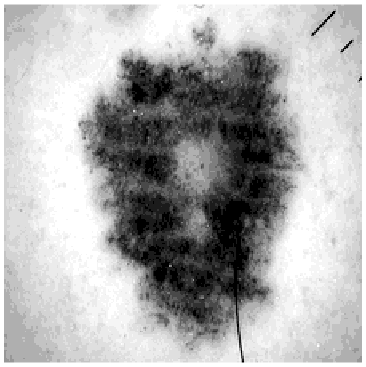
\includegraphics[width=1.7cm]{images/F11-C.png}} & 
        \adjustbox{valign=c}{
\includegraphics[width=1.5cm]{images/F11-D.png}} &
        \adjustbox{valign=c}{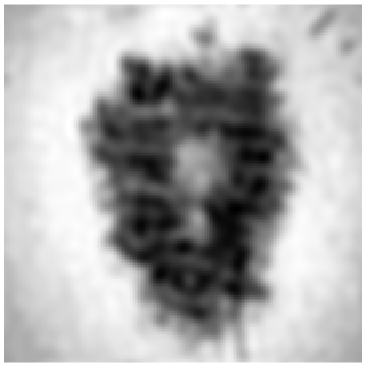
\includegraphics[width=1.7cm]{images/F11-E.png}} & 
        \adjustbox{valign=c}{
\includegraphics[width=1cm]{images/F11-F.png}} \\
        (a) & (b) & (c) & (d) & (e) & (f)\\
    \end{tabular}
    \caption{\footnotesize (a) imagen en el modelo HSI, (b) segmentación de color con K Medias, (c) imagen segmentada en blanco y negro, (d) imagen en blanco y negro con valores ecualizados, (e) imagen con valores ecualizados con trasnformación binaria, (f) imagen con filtro paso bajas.}  
    \label{fig11} 
\end{figure*}

\clearpage

\subsection{Evaluación de desempeño en el modelo HSI}

En el modelo HSI, los colores se definen mediante su tono, saturación e intensidad, aspectos intrínsecamente vinculados a la percepción humana del color \autocite{Rojas:2008}. El propósito de esta sección radica en evaluar de manera subjetiva los efectos resultantes de las manipulaciones de la imagen en comparación con el modelo RGB. Para ello, es necesario obtener una imagen que siga el esquema del modelo HSI. Se hace uso de una función de implementación propia que toma como parámetro una imagen en formato RGB y devuelve la misma imagen en el modelo HSI. En esta función, se lleva a cabo la normalización de los valores de RGB, ajustándolos al rango de 0 a 1. Posteriormente, se procede a descomponer la imagen en sus tres canales de color: R (rojo), G (verde) y B (azul). Se calcula el ángulo theta, que representa la matiz H, mediante una fórmula que incluye las diferencias entre los canales de color.

Se realiza una corrección en el valor de H para asegurar que se encuentre en el rango de 0 a 2 por el valor de pi. La saturación S se determina como 1 menos el valor mínimo entre los tres canales, dividido por la suma de los tres canales. Finalmente, la intensidad I se obtiene como el promedio de los valores de los canales R, G y B. En la última etapa, se utiliza la función ''cat'' para combinar los resultados de H, S e I en una nueva imagen en formato HSI.

 \begin{lstlisting}[style=Matlab-editor, caption=Fragmento del algoritmo K Means, basicstyle=\fontsize{8}{12}\selectfont]
function hsi = rgbTohsi(rgb)
    rgb = double(rgb) / 255;
    r = rgb(:,:,1);
    g = rgb(:,:,2);
    b = rgb(:,:,3);

    num = 0.5 * ((r - g) + (r - b));
    den = sqrt((r - g).^2 + (r - b).*(g - b));
    theta = acos(num ./ (den + eps));

    h = theta;
    h(b > g) = 2*pi - h(b > g); 
    h = h / (2*pi);
 
    s = 1 - 3 * min(rgb, [], 3) ./ sum(rgb, 3);
    i = (r + g + b) / 3;
    hsi = cat(3, h, s, i);
end
\end{lstlisting}

La (Figura~\ref{fig12}) muestra la representación visual del objeto de estudio, conforme al nuevo modelo de color que se ha empleado a lo largo del presente escrito. En (Figura~\ref{fig13}) a (Figura~\ref{fig17}) se detallan los resultados derivados de la aplicación de los procedimientos aludidos en este nuevo espacio cromático. A pesar de la congruencia observada en ciertas instancias, en otras, la semejanza tonal compromete la eficacia de los algoritmos para alcanzar los propósitos iniciales delineados.


\begin{figure}
		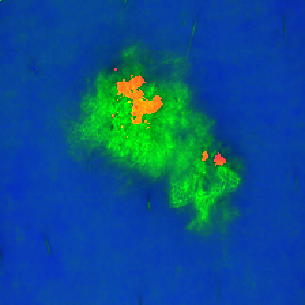
\includegraphics[width=4cm]{images/F12.png} 
\caption{Melanoma maligno representado en el espacio HSI con una resolución de 224 x 244 píxeles almacenado en formato jpg.}
\label{fig12}
\end{figure}

 
% FIGURA 13
\begin{figure*}
    \centering
    \begin{tabular}{cccccccc}
        \adjustbox{valign=c}{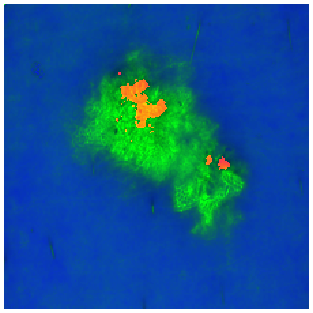
\includegraphics[width=1.5cm]{images/F13-A.png}} &
        \adjustbox{valign=c}{\includegraphics[width=1.5cm]{images/F13-B.png}} & 
        \adjustbox{valign=c}{\includegraphics[width=1.5cm]{images/F13-C.png}} & 
        \adjustbox{valign=c}{\includegraphics[width=1.5cm]{images/F13-D.png}} &
        \adjustbox{valign=c}{\includegraphics[width=1.5cm]{images/F13-E.png}} & 
        \adjustbox{valign=c}{\includegraphics[width=1.5cm]{images/F13-E.png}} & 
		\adjustbox{valign=c}{\includegraphics[width=1.5cm]{images/F13-F.png}} & 
        \adjustbox{valign=c}{\includegraphics[width=1.5cm]{images/F13-G.png}} \\
        (a) & (b) & (c) & (d) & (e) & (f) & (g) & (h)\\
    \end{tabular}
    \caption{\footnotesize A: imagen en el modelo HSI, B: segmentación de color con K Menas, C: imagen segmentada en blanco y negro, D: imagen en blanco y negro con valores ecualizados, E: imagen binaria de D, E: imagen con filtro paso bajas de C, F: imagen binaria de E, G: imagen con filtro butterworth de orden 10 y frecuencia de corte 20,H: imagen binaria de G}  
    \label{fig13} 
\end{figure*}

% FIGURA 14
\begin{figure*}
    \centering
    \begin{tabular}{cccccccc}
        \adjustbox{valign=c}{\includegraphics[width=1.5cm]{images/F14-A.png}} &
        \adjustbox{valign=c}{\includegraphics[width=1.5cm]{images/F14-B.png}} & 
        \adjustbox{valign=c}{\includegraphics[width=1.5cm]{images/F14-C.png}} & 
        \adjustbox{valign=c}{\includegraphics[width=1.5cm]{images/F14-D.png}} &
        \adjustbox{valign=c}{\includegraphics[width=1.5cm]{images/F14-E.png}} & 
        \adjustbox{valign=c}{\includegraphics[width=1.5cm]{images/F14-E.png}} & 
		\adjustbox{valign=c}{\includegraphics[width=1.5cm]{images/F14-F.png}} & 
        \adjustbox{valign=c}{\includegraphics[width=1.5cm]{images/F14-G.png}} \\
        (a) & (b) & (c) & (d) & (e) & (f) & (g) & (h)\\
    \end{tabular}
    \caption{\footnotesize (a) imagen en el modelo HSI, (b) segmentación de color con K Menas, (c) imagen segmentada en blanco y negro, (d) imagen en blanco y negro con valores ecualizados, E: imagen binaria de d, (e) imagen con filtro paso bajas de c, (f) imagen binaria de e, (g) imagen con filtro butterworth de orden 10 y frecuencia de corte 20, (h) imagen binaria de g.}  
    \label{fig14} 
\end{figure*}



% FIGURA 15
\begin{figure*}
    \centering
    \begin{tabular}{cccccccc}
        \adjustbox{valign=c}{\includegraphics[width=1.5cm]{images/F15-A.png}} &
        \adjustbox{valign=c}{\includegraphics[width=1.5cm]{images/F15-B.png}} & 
        \adjustbox{valign=c}{\includegraphics[width=1.5cm]{images/F15-C.png}} & 
        \adjustbox{valign=c}{\includegraphics[width=1.5cm]{images/F15-D.png}} &
        \adjustbox{valign=c}{\includegraphics[width=1.5cm]{images/F15-E.png}} & 
        \adjustbox{valign=c}{\includegraphics[width=1.5cm]{images/F15-E.png}} & 
		\adjustbox{valign=c}{\includegraphics[width=1.5cm]{images/F15-F.png}} & 
        \adjustbox{valign=c}{\includegraphics[width=1.5cm]{images/F15-G.png}} \\
        (a) & (b) & (c) & (d) & (e) & (f) & (g) & (h)\\
    \end{tabular}
    \caption{\footnotesize (a) imagen en el modelo HSI, (b) segmentación de color con K Menas, (c) imagen segmentada en blanco y negro, (d) imagen en blanco y negro con valores ecualizados, E: imagen binaria de d, (e) imagen con filtro paso bajas de c, (f) imagen binaria de e, (g) imagen con filtro butterworth de orden 10 y frecuencia de corte 20, (h) imagen binaria de g.}  
    \label{fig15} 
\end{figure*}

% FIGURA 16
\begin{figure*}
    \centering
    \begin{tabular}{cccccccc}
        \adjustbox{valign=c}{\includegraphics[width=1.5cm]{images/F16-A.png}} &
        \adjustbox{valign=c}{\includegraphics[width=1.5cm]{images/F16-B.png}} & 
        \adjustbox{valign=c}{\includegraphics[width=1.5cm]{images/F16-C.png}} & 
        \adjustbox{valign=c}{\includegraphics[width=1.5cm]{images/F16-D.png}} &
        \adjustbox{valign=c}{\includegraphics[width=1.5cm]{images/F16-E.png}} & 
        \adjustbox{valign=c}{\includegraphics[width=1.5cm]{images/F16-E.png}} & 
		\adjustbox{valign=c}{\includegraphics[width=1.5cm]{images/F16-F.png}} & 
        \adjustbox{valign=c}{\includegraphics[width=1.5cm]{images/F16-G.png}} \\
        (a) & (b) & (c) & (d) & (e) & (f) & (g) & (h)\\
    \end{tabular}
    \caption{\footnotesize (a) imagen en el modelo HSI, (b) segmentación de color con K Menas, (c) imagen segmentada en blanco y negro, (d) imagen en blanco y negro con valores ecualizados, E: imagen binaria de d, (e) imagen con filtro paso bajas de c, (f) imagen binaria de e, (g) imagen con filtro butterworth de orden 10 y frecuencia de corte 20, (h) imagen binaria de g.}   
    \label{fig16} 
\end{figure*}

% FIGURA 17
\begin{figure*}
    \centering
    \begin{tabular}{cccccccc}
        \adjustbox{valign=c}{\includegraphics[width=1.5cm]{images/F17-A.png}} &
        \adjustbox{valign=c}{\includegraphics[width=1.5cm]{images/F17-B.png}} & 
        \adjustbox{valign=c}{\includegraphics[width=1.5cm]{images/F17-C.png}} & 
        \adjustbox{valign=c}{\includegraphics[width=1.5cm]{images/F17-D.png}} &
        \adjustbox{valign=c}{\includegraphics[width=1.5cm]{images/F17-E.png}} & 
        \adjustbox{valign=c}{\includegraphics[width=1.5cm]{images/F17-E.png}} & 
		\adjustbox{valign=c}{\includegraphics[width=1.5cm]{images/F17-F.png}} & 
        \adjustbox{valign=c}{\includegraphics[width=1.5cm]{images/F17-G.png}} \\
        (a) & (b) & (c) & (d) & (e) & (f) & (g) & (h)\\
    \end{tabular}
    \caption{\footnotesize (a) imagen en el modelo HSI, (b) segmentación de color con K Menas, (c) imagen segmentada en blanco y negro, (d) imagen en blanco y negro con valores ecualizados, E: imagen binaria de d, (e) imagen con filtro paso bajas de c, (f) imagen binaria de e, (g) imagen con filtro butterworth de orden 10 y frecuencia de corte 20, (h) imagen binaria de g.}  
    \label{fig17} 
\end{figure*}


\clearpage